% Created by tikzDevice version 0.12.3 on 2019-12-18 13:31:18
% !TEX encoding = UTF-8 Unicode
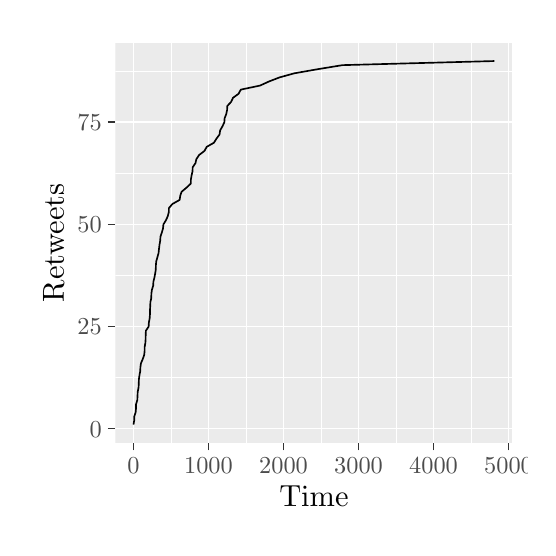
\begin{tikzpicture}[x=1pt,y=1pt]
\definecolor{fillColor}{RGB}{255,255,255}
\path[use as bounding box,fill=fillColor,fill opacity=0.00] (0,0) rectangle (180.67,180.67);
\begin{scope}
\path[clip] (  0.00,  0.00) rectangle (180.67,180.67);
\definecolor{drawColor}{RGB}{255,255,255}
\definecolor{fillColor}{RGB}{255,255,255}

\path[draw=drawColor,line width= 0.6pt,line join=round,line cap=round,fill=fillColor] (  0.00,  0.00) rectangle (180.68,180.68);
\end{scope}
\begin{scope}
\path[clip] ( 31.71, 30.69) rectangle (175.17,175.17);
\definecolor{fillColor}{gray}{0.92}

\path[fill=fillColor] ( 31.71, 30.69) rectangle (175.17,175.17);
\definecolor{drawColor}{RGB}{255,255,255}

\path[draw=drawColor,line width= 0.3pt,line join=round] ( 31.71, 54.23) --
	(175.17, 54.23);

\path[draw=drawColor,line width= 0.3pt,line join=round] ( 31.71, 91.12) --
	(175.17, 91.12);

\path[draw=drawColor,line width= 0.3pt,line join=round] ( 31.71,128.02) --
	(175.17,128.02);

\path[draw=drawColor,line width= 0.3pt,line join=round] ( 31.71,164.92) --
	(175.17,164.92);

\path[draw=drawColor,line width= 0.3pt,line join=round] ( 51.78, 30.69) --
	( 51.78,175.17);

\path[draw=drawColor,line width= 0.3pt,line join=round] ( 78.89, 30.69) --
	( 78.89,175.17);

\path[draw=drawColor,line width= 0.3pt,line join=round] (106.00, 30.69) --
	(106.00,175.17);

\path[draw=drawColor,line width= 0.3pt,line join=round] (133.11, 30.69) --
	(133.11,175.17);

\path[draw=drawColor,line width= 0.3pt,line join=round] (160.22, 30.69) --
	(160.22,175.17);

\path[draw=drawColor,line width= 0.6pt,line join=round] ( 31.71, 35.78) --
	(175.17, 35.78);

\path[draw=drawColor,line width= 0.6pt,line join=round] ( 31.71, 72.67) --
	(175.17, 72.67);

\path[draw=drawColor,line width= 0.6pt,line join=round] ( 31.71,109.57) --
	(175.17,109.57);

\path[draw=drawColor,line width= 0.6pt,line join=round] ( 31.71,146.47) --
	(175.17,146.47);

\path[draw=drawColor,line width= 0.6pt,line join=round] ( 38.23, 30.69) --
	( 38.23,175.17);

\path[draw=drawColor,line width= 0.6pt,line join=round] ( 65.34, 30.69) --
	( 65.34,175.17);

\path[draw=drawColor,line width= 0.6pt,line join=round] ( 92.45, 30.69) --
	( 92.45,175.17);

\path[draw=drawColor,line width= 0.6pt,line join=round] (119.55, 30.69) --
	(119.55,175.17);

\path[draw=drawColor,line width= 0.6pt,line join=round] (146.66, 30.69) --
	(146.66,175.17);

\path[draw=drawColor,line width= 0.6pt,line join=round] (173.77, 30.69) --
	(173.77,175.17);
\definecolor{drawColor}{RGB}{0,0,0}

\path[draw=drawColor,line width= 0.6pt,line join=round] ( 38.23, 37.25) --
	( 38.50, 38.73) --
	( 38.52, 40.21) --
	( 39.02, 41.68) --
	( 39.15, 43.16) --
	( 39.17, 44.63) --
	( 39.62, 46.11) --
	( 39.69, 47.58) --
	( 39.76, 49.06) --
	( 40.06, 50.54) --
	( 40.15, 52.01) --
	( 40.18, 53.49) --
	( 40.37, 54.96) --
	( 40.65, 56.44) --
	( 40.73, 57.92) --
	( 40.94, 59.39) --
	( 41.56, 60.87) --
	( 42.09, 62.34) --
	( 42.26, 63.82) --
	( 42.27, 65.30) --
	( 42.53, 66.77) --
	( 42.63, 68.25) --
	( 42.64, 69.72) --
	( 42.73, 71.20) --
	( 43.71, 72.67) --
	( 43.80, 74.15) --
	( 44.08, 75.63) --
	( 44.19, 77.10) --
	( 44.20, 78.58) --
	( 44.28, 80.05) --
	( 44.35, 81.53) --
	( 44.67, 83.01) --
	( 44.69, 84.48) --
	( 44.89, 85.96) --
	( 45.35, 87.43) --
	( 45.43, 88.91) --
	( 45.80, 90.39) --
	( 46.08, 91.86) --
	( 46.30, 93.34) --
	( 46.32, 94.81) --
	( 46.48, 96.29) --
	( 46.89, 97.76) --
	( 47.30, 99.24) --
	( 47.45,100.72) --
	( 47.63,102.19) --
	( 47.88,103.67) --
	( 47.98,105.14) --
	( 48.47,106.62) --
	( 48.90,108.10) --
	( 49.04,109.57) --
	( 49.95,111.05) --
	( 50.61,112.52) --
	( 51.00,114.00) --
	( 51.04,115.48) --
	( 52.29,116.95) --
	( 54.91,118.43) --
	( 55.13,119.90) --
	( 55.63,121.38) --
	( 57.38,122.85) --
	( 58.95,124.33) --
	( 58.98,125.81) --
	( 59.22,127.28) --
	( 59.57,128.76) --
	( 59.62,130.23) --
	( 60.63,131.71) --
	( 60.96,133.19) --
	( 61.95,134.66) --
	( 63.89,136.14) --
	( 64.70,137.61) --
	( 67.30,139.09) --
	( 68.22,140.57) --
	( 69.32,142.04) --
	( 69.53,143.52) --
	( 70.36,144.99) --
	( 71.07,146.47) --
	( 71.16,147.94) --
	( 71.75,149.42) --
	( 72.06,150.90) --
	( 72.13,152.37) --
	( 73.52,153.85) --
	( 74.19,155.32) --
	( 76.23,156.80) --
	( 77.00,158.28) --
	( 83.97,159.75) --
	( 87.21,161.23) --
	( 91.02,162.70) --
	( 96.37,164.18) --
	(104.79,165.66) --
	(113.76,167.13) --
	(168.65,168.61);
\end{scope}
\begin{scope}
\path[clip] (  0.00,  0.00) rectangle (180.67,180.67);
\definecolor{drawColor}{gray}{0.30}

\node[text=drawColor,anchor=base east,inner sep=0pt, outer sep=0pt, scale=  0.88] at ( 26.76, 32.75) {0};

\node[text=drawColor,anchor=base east,inner sep=0pt, outer sep=0pt, scale=  0.88] at ( 26.76, 69.64) {25};

\node[text=drawColor,anchor=base east,inner sep=0pt, outer sep=0pt, scale=  0.88] at ( 26.76,106.54) {50};

\node[text=drawColor,anchor=base east,inner sep=0pt, outer sep=0pt, scale=  0.88] at ( 26.76,143.44) {75};
\end{scope}
\begin{scope}
\path[clip] (  0.00,  0.00) rectangle (180.67,180.67);
\definecolor{drawColor}{gray}{0.20}

\path[draw=drawColor,line width= 0.6pt,line join=round] ( 28.96, 35.78) --
	( 31.71, 35.78);

\path[draw=drawColor,line width= 0.6pt,line join=round] ( 28.96, 72.67) --
	( 31.71, 72.67);

\path[draw=drawColor,line width= 0.6pt,line join=round] ( 28.96,109.57) --
	( 31.71,109.57);

\path[draw=drawColor,line width= 0.6pt,line join=round] ( 28.96,146.47) --
	( 31.71,146.47);
\end{scope}
\begin{scope}
\path[clip] (  0.00,  0.00) rectangle (180.67,180.67);
\definecolor{drawColor}{gray}{0.20}

\path[draw=drawColor,line width= 0.6pt,line join=round] ( 38.23, 27.94) --
	( 38.23, 30.69);

\path[draw=drawColor,line width= 0.6pt,line join=round] ( 65.34, 27.94) --
	( 65.34, 30.69);

\path[draw=drawColor,line width= 0.6pt,line join=round] ( 92.45, 27.94) --
	( 92.45, 30.69);

\path[draw=drawColor,line width= 0.6pt,line join=round] (119.55, 27.94) --
	(119.55, 30.69);

\path[draw=drawColor,line width= 0.6pt,line join=round] (146.66, 27.94) --
	(146.66, 30.69);

\path[draw=drawColor,line width= 0.6pt,line join=round] (173.77, 27.94) --
	(173.77, 30.69);
\end{scope}
\begin{scope}
\path[clip] (  0.00,  0.00) rectangle (180.67,180.67);
\definecolor{drawColor}{gray}{0.30}

\node[text=drawColor,anchor=base,inner sep=0pt, outer sep=0pt, scale=  0.88] at ( 38.23, 19.68) {0};

\node[text=drawColor,anchor=base,inner sep=0pt, outer sep=0pt, scale=  0.88] at ( 65.34, 19.68) {1000};

\node[text=drawColor,anchor=base,inner sep=0pt, outer sep=0pt, scale=  0.88] at ( 92.45, 19.68) {2000};

\node[text=drawColor,anchor=base,inner sep=0pt, outer sep=0pt, scale=  0.88] at (119.55, 19.68) {3000};

\node[text=drawColor,anchor=base,inner sep=0pt, outer sep=0pt, scale=  0.88] at (146.66, 19.68) {4000};

\node[text=drawColor,anchor=base,inner sep=0pt, outer sep=0pt, scale=  0.88] at (173.77, 19.68) {5000};
\end{scope}
\begin{scope}
\path[clip] (  0.00,  0.00) rectangle (180.67,180.67);
\definecolor{drawColor}{RGB}{0,0,0}

\node[text=drawColor,anchor=base,inner sep=0pt, outer sep=0pt, scale=  1.10] at (103.44,  7.64) {Time};
\end{scope}
\begin{scope}
\path[clip] (  0.00,  0.00) rectangle (180.67,180.67);
\definecolor{drawColor}{RGB}{0,0,0}

\node[text=drawColor,rotate= 90.00,anchor=base,inner sep=0pt, outer sep=0pt, scale=  1.10] at ( 13.08,102.93) {Retweets};
\end{scope}
\end{tikzpicture}
